\chapter{Introduction}
\label{cha:introduction}
% Start with a general context;
% General problem;
% Then, DZ2


\section{Context}
% Global warming
% ICT role
% Renewable energy in data centers
% Uncertainties

Global warming is one of the biggest challenges humanity is facing. A recent rapport shows that we are walking toward a global mean temperature increase by 2100 of 2.7°C, well above the 1.5°C defined by the Paris Agreement \cite{tracker2022massive}. The same rapport predicts the rise in mean global temperature will be around 1.8°C even after implementing all announced Paris Agreement goals. Achieving 1.5°C demands an engagement of all sectors to reduce greenhouse gas (GHG) emissions. One significant greenhouse gas (GHG) emitter is the Information and Communications Technology (ICT) sector. It produces around 1.8-2.8\% of the world's total GHG \cite{freitag2021climate}. Inside ICT, Data centers and transmission networks are responsible for nearly 1\% of energy-related GHG emissions \cite{centres2022data}. Due to its uninterrupted operation, the data centers sector is one of the most electricity-expensive ICT actors. A report revealed that Google data centers consumed the same amount of energy as the entire city of San Francisco in 2015 \cite{khan2018exploiting}. In addition, the situation tends to get even worse due to the improvements reduction in processor technologies and the predicted expansion of internet usage \cite{cisco2020cisco, freitag2021climate}.

Big cloud providers such as Google and Amazon are trying to reduce energy consumption and increase the power coming from renewable sources (RES) \cite{Masanet984}. Renewable sources generate energy coming from clean sources such as wind and solar \cite{rostirolla2022survey}. A significant drawback of RES is they are highly dependent on weather conditions, creating power intermittence. These providers smooth this intermittence by not migrating entirely to RES, maintaining a connection to the grid \cite{rostirolla2022survey}. Therefore, they are not 100\% clean. A renewable-only data center must consider this intermittence in its decision-making. Another source of uncertainty comes from the user's demand. A data center receives requests continuously, and providing high availability is a challenge for a renewable-only data center.

A way to reduce the impact of RES power production intermittence is by adding storage elements \cite{rostirolla2022survey}. Batteries and hydrogen tanks can shift generation and/or consumption over time. A renewable-only data center demands a massive storage capacity \cite{rostirolla2022survey}. For example, Google plans to use energy from 350 MW solar panels connected to a storage system with 280 MW \cite{branscombe2020google}. While helping to deal with RES intermittence, storage management introduces another level of decision. For example, it can store energy during the day using at night. Nevertheless, the demand during the day could be higher than at night, so maybe it is better to use the energy during the day. Therefore, this is another big challenge for migrating to a 100\% clean data center.

Some works propose ways to deal with both demand and weather uncertainties using predictions \cite{wiesner2022cucumber, haddad2019mixed, lu_energy-efficient_2018, goiri2015matching}. Forecasting the upcoming requests and the weather helps to plan storage usage. They use these predictions to maximize renewable usage but with the grid as backup. All these works are valuable and important to optimize renewable usage. However, the forecast can vary from the actual values. Other works focus on reacting to real events \cite{liu2023online, he2022online, caux2019phase, sharma2011blink}. They try to minimize the data center operational cost, maximize renewable usage, increase the revenue of job execution, or improve the Quality of Service. Usually, they define ways to schedule the jobs, optimizing their objective. However, they focus on short-term decisions without long-term management. Since these works also have the grid as backup, storage management is not a concern. Some works mix predictions with reactive actions. For example, Goiri et al. \cite{goiri2015matching} propose a scheduling algorithm that predicts solar power production and uses it to define the best moment to start new jobs, using brown energy (from the grid) when necessary. Also, Venkataswamy et al. \cite{venkataswamy2023rare} created a job scheduler that defines job placement according to the available machines. The available machines are given by a fixed plan (which can use power from renewable, batteries, or grid), with no modifications.

Few research initiatives are investigating how to design and operate a renewable-only data center. One of them is the ANR Datazero2 project \cite{Datazero}. This project aims to define a feasible architecture to maintain a renewable-only data center. This architecture includes several elements to provide energy to the IT servers, such as Wind turbines, Solar panels, Batteries, and Hydrogen tanks. Considering the decision-making, Datazero2 divides the problem into two parts: offline and online. The offline module predicts power demand and production. Using these predictions and considering long-term constraints, this module creates a power and IT plan for the near future. The online module applies this plan but reacts to the actual events. So, the online module modifies both power and IT decisions. In power decisions, this module defines when to use more or less power from storage. For example, it can use more battery to improve the Quality of Service (QoS) from the jobs. On the IT side, the online module receives the jobs from the users and defines when and where to place them. In this thesis, we focus on the online problem. The goal is to design and prove the efficiency of a novel approach for scheduling users' jobs, using the offline plan as a guide but making changes to improve the QoS.

\section{Problem Statement}
% How to deal with these uncertainties

A data center powered by renewable energy demands several levels of decision. Several works aim to optimize some of these decisions. We can cite demand and production predictions, cost optimization, sizing, shifting demand, battery management, admission control, and job scheduling, to mention a few. Usually, these works introduce a link to the grid, using it as a backup to cope with peak demand. Removing the grid of the context adds several challenges. This context increases the need for predictions to manage weather and workload uncertainties. Another key element in renewable-only data centers is storage. Aligning prediction and storage elements allows it to define the best strategy to handle users' requests. However, actual demand and production can vary from the predictions. So, the online module must react to the actual values. This reaction can improve the QoS (e.g., when there is more production than expected) or reduce the impact of critical events.

Figure \ref{fig:introduction_problem} illustrates all the elements in the decision process. We consider only renewable sources and storage elements without grid connection. An offline optimization gives an offline plan using production and demand prediction. The offline plan has a limited size named time window (e.g., three days). So, offline suggests actions to online during this time window. Online receives the actual renewable production from wind turbines and solar panels. Online adapts storage usage according to the actual production. Since hydrogen has a longer start-up time, it is difficult to manage it in online mode. Therefore, we let hydrogen usage from the offline optimization, using it to provide energy during periods with low renewable production (e.g., during the winter). So, online decides about battery usage only. Battery management introduces two new challenges regarding the Battery's State of Charge (SoC). SoC means the level of charge of a battery relative to its capacity. A good practice to extend the battery's lifetime is to avoid drying or overcharging it \cite{xu2016modeling}. So, maintaining the SoC between reasonable levels is the first challenge. Online has the entire time window to make modifications in battery usage. However, it must finish the time window close to the expected SoC (given by the offline plan). Since the data center runs continuously, it is not viable to dry the batteries every time window. 

\begin{figure}[!htb]
    \centering
    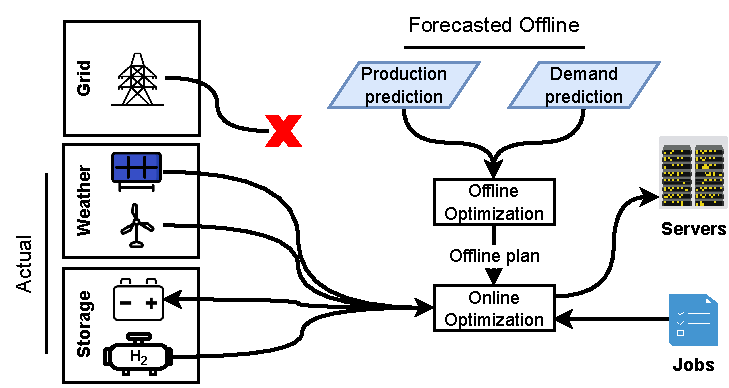
\includegraphics[scale=1]{Images/Introduction/Problem_overview_thesis.pdf}
    \caption{Problem overview. Online receives an offline plan, the actual renewable production, and the users' jobs. It must define storage usage, job placement in the servers, and server speed.}
    \label{fig:introduction_problem}
\end{figure}

On the IT side, online optimization receives the jobs from the users and must schedule them on the available servers. Online has the freedom to turn on, turn off, or change the speed of the servers. Changing the speed of a server is possible due to the Dynamic voltage and frequency scaling (DVFS) technique. DVFS allows servers' speed reduction, spending less energy. However, putting a job on a server with a decreased speed can impact the job QoS. To sum up, online must manage the battery (maintaining the SoC between thresholds and finishing the time window with the battery level close to the target), schedule the jobs, and balance the servers' speed.

This thesis' first objective is to optimize online power decision modifications given by the offline plan, coping with the uncertainty coming from renewable production and workload arrival. The second goal is mixing power and scheduling online decisions, turning the scheduling storage aware. This mix allows the scheduling to make better decisions than usual algorithms. The last objective is to add the predictions to the online decision. Different contributions address these questions in this manuscript.


\section{Main contributions}
% Find the algorithms to deal with the uncertainties, improving QoS
\begin{center}
    \textbf{Proposing a simulation environment}
\end{center}
Aiming to simulate data center management, describing the workload, weather, server configuration, and simulation tool is a crucial step. We detail in Section \ref{cha:model} the simulation environment, providing a framework for future works. Regarding the workload, some traces are used in literature, such as Google \cite{reiss2011google}, Parallel Workloads Archive \cite{feitelson2014experience}, and Alibaba \cite{wang2022characterizing}. We propose filtering in a trace from Parallel Workloads Archive named Metacentrum \cite{klusavcek2017real}. Considering the weather, it is possible to collect data from everywhere in the world. We present the methodology to generate power production from a weather trace. The third input is the server configuration. We demonstrate the data collected from a server in GRID5000\footnote{https://www.grid5000.fr} used in this thesis. Finally, we present the simulation tool named BATSIM\footnote{https://batsim.org/}, based on SIMGRID\footnote{https://simgrid.frama.io/}. We introduced in this simulation tool the modifications needed to manage battery and power production. The ensemble of these data and definitions allows future work inside and outside the Datazero2 project.

\begin{center}
    \textbf{Defining offline power and IT decisions}
\end{center}
As illustrated in Figure \ref{fig:introduction_problem}, an important part is the offline plan. This plan must consider the power and demand predictions to define the actions for the next time window. We demonstrate in Section \ref{cha:model} a model to deal with both predictions. We separate the problem into two parts. First, we present the optimization problem to define power engagement, giving a power prediction. This optimization problem results in expected renewable power production, storage usage, and expected SoC. The sum of the expected renewable power production and storage usage is the power envelope. The second part is the IT servers' state (on/off) and speed definition. Another optimization problem defines the configuration to give the highest speed with the power available in the power envelope. The result of both optimizations is the input for the online module.

\begin{center}
    \textbf{Reacting to power fluctuations}
\end{center}
Given the result of the optimization problem, next, we propose a heuristic to react to the power fluctuations. Since there is no perfect prediction, one source of divergence is the difference between the prediction and actual values. Also, the offline model considers constant server power usage. Finally, the scheduling can modify the battery usage to improve the QoS. The objective is to approximate the state of charge of the target level at the end of the time window. So, for example, a lower-than-expected production demands more power from batteries to maintain the servers at their configuration. Then, online must reduce future battery use. We propose four policies to compensate for these divergences in the power envelope. Each one finds a different moment in the future to place the compensation. 

\begin{center}
    \textbf{Learning the actions to deal with power fluctuations}
\end{center}
After proposing several compensation policies, we implement two Reinforcement Learning (RL) algorithms. We verify that each policy is better in different moments inside the time window. So, we tried to learn the best moment to apply each one. Considering each policy as RL's action, we present the RL's state and reward. We implemented two well-known RL algorithms named Contextual Multi-Armed Bandit and Q-Learning. 

\begin{center}
    \textbf{Defining battery-aware scheduling using production and demand predictions}
\end{center}

Finally, the last contribution is a battery-aware scheduling algorithm. This algorithm is based on the well-known EASY-Backfilling. It considers the server configuration to define job placement. However, it can modify the IT configuration allowing to place jobs. These modifications consider the SoC in decision-making. Regarding power compensations, it creates several possible scenarios of production and demand using the predictions. According to these scenarios, the heuristic finds the best moment to make the compensations. It also uses these scenarios to verify dangerous moments, where it must be careful in the scheduling. This heuristic mixes all decisions providing a well-balanced answer to the online multi-objective problem.

\section{Publications and Communication}

\textbf{Submitted Peer Reviewed Conferences:}
\begin{itemize}
    \item I. F. de Nardin, P. Stolf and S. Caux, ``Adding Battery Awareness in EASY Backfilling'', 2023 IEEE 35th International Symposium on Computer Architecture and High Performance Computing (SBAC-PAD), Porto Alegre, Brazil, 2023.
\end{itemize}

\textbf{Accepted Peer Reviewed Conferences:}
\begin{itemize}
    \item I. F. de Nardin, P. Stolf and S. Caux, ``Analyzing Power Decisions in Data Center Powered by Renewable Sources'', 2022 IEEE 34th International Symposium on Computer Architecture and High Performance Computing (SBAC-PAD), Bordeaux, France, 2022, pp. 305-314;
    \item I. F. de Nardin, P. Stolf and S. Caux, ``Evaluation of Heuristics to Manage a Data Center Under Power Constraints'', 2022 IEEE 13th International Green and Sustainable Computing Conference (IGSC), Pittsburgh, PA, USA, 2022, pp. 1-8;
    \item I. F. de Nardin, P. Stolf and S. Caux, ``Mixing Offline and Online Electrical Decisions in Data Centers Powered by Renewable Sources'', IECON 2022 – 48th Annual Conference of the IEEE Industrial Electronics Society, Brussels, Belgium, 2022, pp. 1-6;
    \item  I. F. de Nardin, P. Stolf and S. Caux, ``Smart Heuristics for Power Constraints in Data Centers Powered by Renewable Sources'', Conférence francophone d'informatique en Parallélisme, Architecture et Système (COMPAS 2022), Jul 2022, Amiens, France. paper 7.
\end{itemize}

\textbf{Others Disseminations:}
\begin{itemize}
    \item Talk: Analyzing Power Decisions in Data Center
    Powered by Renewable Sources, GreenDays@Lyon, March 2023.
\end{itemize}

\section{Dissertation Outline}
The remaining dissertation has the following organization:
\begin{itemize}
    \item[] \textbf{Chapter 2 - Context and Related Work:} This chapter presents the fundamentals to understand this dissertation. Considering the scope of the topic, the context consists of four parts. First, we introduce the context of global and ICT GHG emissions. Then, we describe renewable energy as an alternative to replace brown energy. After, we explain the usage of renewable to power a data center. Then, we define the uncertainties of weather and workload in a renewable-only data center. This last part also clarifies the importance of using predictions but with an online adaptation. After presenting the context, we introduce a list of works that solve part of our problem, highlighting the existing gaps in the state-of-the-art;
    \item[] \textbf{Chapter 3 - Modelling, Data, and Simulation:} In this chapter, we describe the model to deal with the several elements that compose a renewable-only data center. Datazero2 creates a division between Offline and Online decisions. We present the model to deal with offline decisions using predicted power demand and production. Then, we demonstrate the output of Offline used by the Online. Finally, we define the Online model, which englobes the job scheduling and modifications in the Offline plan. After describing the model, we explain the source of the different data (e.g., workload, weather, servers) applied in the simulations. We present an explanation of the work done in the traces of the literature. Finally, we present the simulation tools used in this work;
    \item[] \textbf{Chapter 4 - Introducing Power Compensations:} This chapter describes the proposed optimization to react to power uncertainties. We created four heuristics to find the best place to compensate for battery changes, which aim to reduce the number of killed jobs and the distance between the battery level and the target level. The results presented are related to the publications \cite{de2022mixing} and \cite{de2022analyzing};
    \item[] \textbf{Chapter 5 - Learning Power Compensations:} This chapter presents the idea and the results of the introduction of Reinforcement Learning (RL) in the power compensation problem. We propose two RL algorithms (Q-Learning and Contextual Multi-Armed Bandit) to learn the best moment to compensate;
    \item[] \textbf{Chapter 6 - Adding Battery Awareness in EASY Backfilling:} This chapter explains a heuristic to mix scheduling and power compensation decisions. This heuristic is based on the EASY Backfilling scheduling algorithm but considers the battery's State of Charge to make better decisions;
    % \item[] \textbf{Chapter 7 - Middleware Integration:} This chapter presents the tools, frameworks, and approaches applied to integrate the algorithms in the Datazero2 middleware. Also, we describe the work done to create a docker environment, allowing different actors to execute the middleware;
    \item[] \textbf{Chapter 7 - Conclusion and Perspectives:} Finally, in this chapter, we summarize the contributions of this work, providing a discussion about future works.
\end{itemize}
